\documentclass[oneside]{book}
\usepackage[utf8]{inputenc}
\usepackage{float}
\usepackage{graphicx}
\usepackage{amsmath}
\usepackage{color}
\usepackage{multicol}
\usepackage{ragged2e}
\usepackage{listings}
\usepackage{pdfpages}
\title{Notes de Cours INF 3610}
\date{2018-10-10}
\author{Olivier Sirois}
\setlength\parindent{0pt}
\makeindex
\pagenumbering{arabic}
\begin{document}
    \setcounter{page}{1}
    \maketitle
    \tableofcontents
    \chapter{Cours 1,2 - Introduction}
    Quelques définitions:\\
    
    \section{Systeme temps réelle}
    Contraintes de temps très importantes, elle fait normalement partie des spécifications et doivent absolument être respecté. Normalement on parle d'un environnnement qui agit sur des capteurs (senseurs) avec le système qui agit de facon correcte à ces stimuli dans un temps donné.\\
    
    Les systèmes temps réelle sont normalment composé de deux sous-systèmes:
    \begin{itemize}
        \item contrôleur (PC ou microControleur)
        \item contrôlé (environnement physique)
    \end{itemize}

    La relation entre les deux sous-système est décrite par trois opérations
    \begin{itemize}
        \item échantillonnage
        \item calcule
        \item réponse
    \end{itemize}

    On différencie aussi entre les contraintes dure et les contraintes douces. Normalement, il est critique de devoir respecté les contriantes dure tandis que pour les contraintes c'est un peu plus flexible.
    \paragraph{def des slides}
    Un systeme qui doit repondre a un stimuli provaenant d'un environnement dans un temps donnée.\\
    
    \section{Systeme embarquée}
    Un système embarqué est un système autonome, souvent temps réelle, servant à résoudre des fonctions et des tâches spéficique et disposant de resources limités. c'est limité parce que normalement on essaie de réduire les couts parce qu'on veut en faire une production industriel.\\
    
    La complexité peut varier, c'Est pas la même chose entre un lave-vaisselle et un contrôleur de missile. Normalement, on utilise du matériel pour la performance et la consommation tandis qu'on utilise du logiciel pour la flexibilité.\\
    
    \subsection{contraintes}
    Normalement, les métriques de conception d'un système embarqué sont :
    \begin{itemize}
        \item Taille
        \item fiabilité
        \item Consommation et dissipation de puissance
        \item cout de production
        \item temps de commercialisation (time to market)
    \end{itemize}

    On peut aussi avoir d'autre contrainte, genre:
    \begin{itemize}
        \item Tolérance aux pannes
        \item Résistance aux chocs et temp.
        \item BIST - built in self test. Pouvoir se diagnostiquer automatiquement
        \item Flexibilité et mise-a jour
    \end{itemize}

    Normalement, les systèmes embarqués sont utilisé dans un environnement réactif ou dans des situation très demandant.
    
    \section{Class d'application}
    \begin{itemize}
        \item \textbf{Systèmes dominé par le contrôle - contrôle sophistiqué} - Requiert des contrainte de temps, de temps dure(critical failure) et mêmes plusieurs tâche simultané (multitache, concurrence, changement de contexte rapide requis >1us).\\
        
        Normalement, il y a peu de données associsé à chaque machine à états. On peut normalement associer la mémoire sur puces à ces machine pour accélérer le changement de contexte.\\
        
        Un RTOS préemptif est généralement requis, c-a-d. un OS qui a un ordonnancement de tâche sophistiqué qui tache les plus prioritaire en premier. Plusieur algorithme d'ordonnancement existe pour ces OS\\
        
        \item \textbf{Systèmes dominés par les données - contrôle qui traite une quantité importante de données.} - À certaine caractéristique:
        \begin{itemize}
            \item Beaucoup de MIPS ou de MFLOPS
            \item bande passante élevé
            \item instruction spécialisé pour DSP
            \item Support limité pour les interruptions et les changements de contexte
            \item beaucoup de données pour un même contexte
            \item très peu de changement de contexte son nécessaire car un seul flot de données mais à grand débit
        \end{itemize}
    \end{itemize}
    
    \section{Noyau RTOS}
    \subsection{Système avant/arrière-plan vs système multitache}
    \subsubsection{Arrière plan}
    s'applique normalement à des système peu complexe ou de petites tailles. C'est généralement une boucle infini qui appel à tour de rôle différent modules. La gestion des événements est généralement asynchrones (ISR). On peut avoir des interruptions de minuteur ou par I/O.On retrouve normalement cette méthode dans les systèmes de petite tailles (petit processeur). Cette approche est simple, mais elle très peu modulaire.\\

    \begin{figure}[!ht]
    	\centering
    	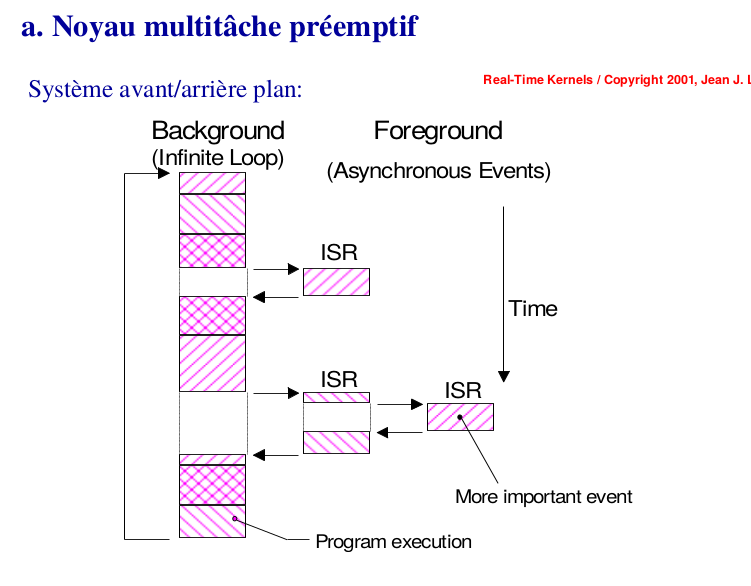
\includegraphics[width=8cm, height = 8cm, keepaspectratio]{Images/avantarriereplan.png}
    	\caption{Système avant-arrière plan}
    	\label{fig:Foreground-Background}
    \end{figure}
    
    \subsection{Systeme multi-tache}
    S'applique généralement a des systeme plus complexes. Elle favorise la réutilisation du code de par sa modularité. On donne accès à des outils évolués (Flgas, mutex, sémaphore, MB, Q). sa permet d'augmenter l'abstraction lors de la conception et exploite le concept de tâche et de programmation concurrente. (linux kernel).\\
    
    Contrairement au systèmes types arriere/avant-plan, ces systèmes sont super modulaires. Un des désavantages est que sa prend un système massif/complexe et beaucoup de temps de développement. C'est très gourmand en mémoire alors sa peut être à reconsidérer dépendament de ton hardware.\\
    
    \begin{figure}[!ht]
  	\centering
  	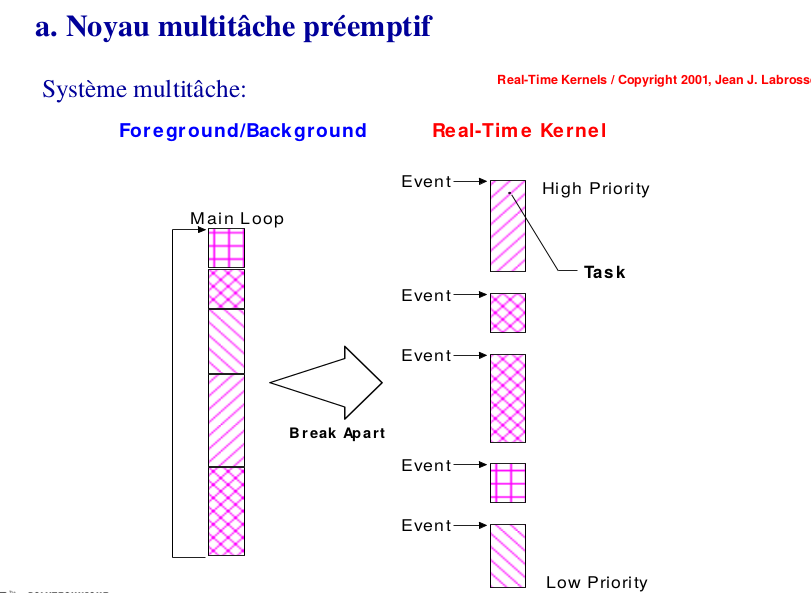
\includegraphics[width=8cm, height = 8cm, keepaspectratio]{Images/multitache.png}
  	\caption{Système multitâche}
  	\label{fig:Multitache}
	\end{figure}  
 
    \textbf{tâche} Un simple programme évoluant comme si il avait le CPU pour lui-même. Typiquement une boucle infini dans un des états suivant:...\\
    \subsubsection{Noyau préemptif}
    un système préemptif est un système ou les tâches peuvent utiliser des fonctions non réentrantes (excepté pour la syncronisation avec les ISR)\\
    
    la latence d'interruption est relativement faible. Sa exploite moins les mutex et les sémaphores. Par contre ça l'a le désavantage d'être relativement moins performant.\\
    
    En générale, les système préemptif ne sont pas utilisé dans les systèmes embarqués.\\
    
    Le paradigme est privilégié. Normalement sont des systèmes super réactif ou les tâches prioritaire s'exécutent en premier.\\
    
    
    \begin{figure}[!ht]
    	\centering
    	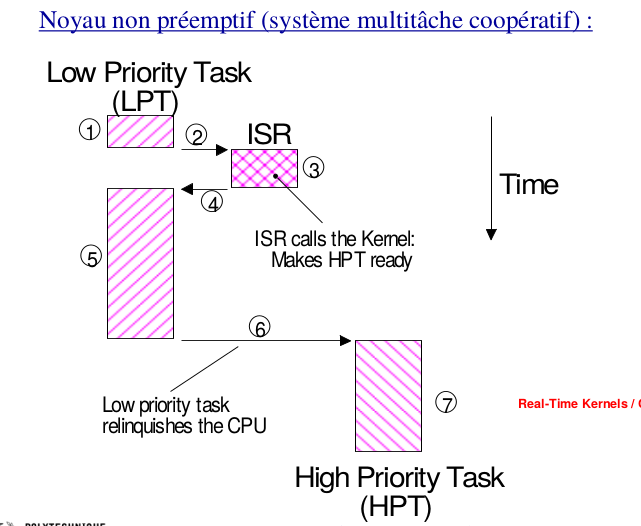
\includegraphics[width=8cm, height = 8cm, keepaspectratio]{Images/noyau_non_preemptif.png}
    	\caption{Exemple d'un noyau non-Preemptif}
    	\label{fig:NoyauNonPreemptif}
    \end{figure}
    
    \subsubsection{Priorité}
    Détermine l'exécution des tâches. c'est une métrique caractérisant son importance. Les tâches prioritaire vont être exécuter avant ceux moins prioritaire. Normalement on représente sont importance avec un numéro, ce numéro peut être assigner au lancement de la tâche mais peut aussi être changer durant son exécution.\\
    
    
    
    \subsubsection{Programmation concurrente}
    Normalement utilité our exprimer le potentiel parallélisme et pour gérer les problème de synchronisation et de communication dans les systèmes multi-tâches.\\
    
    \begin{figure}[!ht]
    	\centering
    	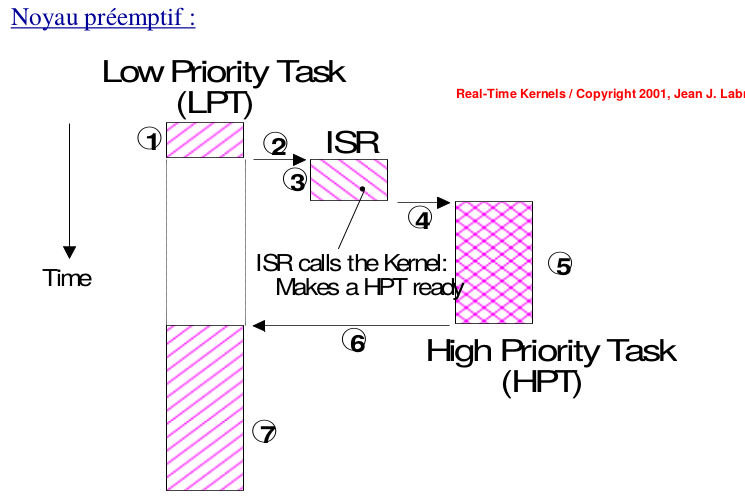
\includegraphics[width=8cm, height = 8cm, keepaspectratio]{Images/noyau_preemptif.png}
    	\caption{Exemple d'un noyau Preemptif}
    	\label{fig:NoyauPreemptif}
    \end{figure}

    \subsubsection{Ressources partagées}
    Techniquement, une ressource partagée est une ressources utilités par plus d'une tâche, simultanément ou non.\\
    
    
    La programmation concurrente introduis nécessairement le problème de partage des ressources. Une ressource est entité exploité par une tâche. Elle peut etre corrompu si elle est simultanément utilisé, ce qui va inévitablement crasher.. \\
    
    Pour partager les ressources, on chercher nécessairement a avoir une fonction réentrante. une fonction qui peut etre appelé par plus d'une tâche sans crainte de corrompre les données (threadsafe).\\
    
    Pour s'assurer qu'une fonction soit réentrante, on s'assure généralement que les variables sont le plus souvent locals que possible.\\
    
    On exploite les mutex/sémaphores lors de partage de variables.\\
    
    Désactiver les interruptions ou le scheduleur.. (pas recommander).\\
    
    Afin d'éviter la corruption de données, nous utilisons des fonctions \textbf{réentrantes} pour régler le problème. L'approche recommandé est d'utiliser des sémaphore/mutex\\
    

    \begin{figure}[!ht]
    	\centering
    	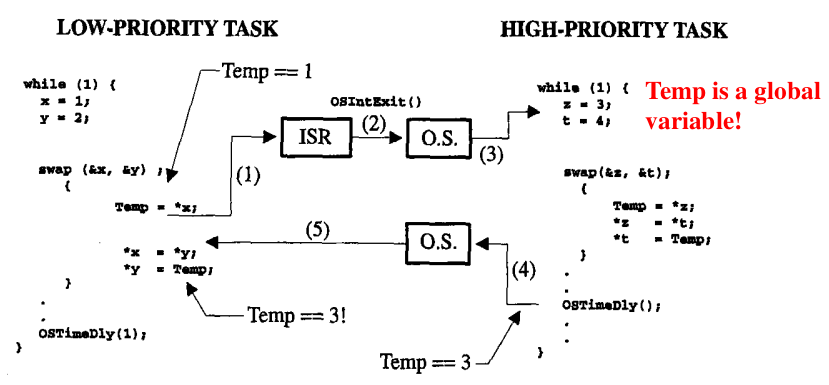
\includegraphics[width=8cm, height = 8cm, keepaspectratio]{Images/fonction_non_reentrante.png}
    	\caption{Fonction non reentrante}
    	\label{fig:FonctionNonReentrante}
    \end{figure}

    \textbf{Sections critiques}
    Une section est dite critique si elle doit etre exécuter sans être interrompus. Ce qui pourrait causer un deadlock.. ou un traitement de données incorrect.
    
    \subsubsection{Sémaphores}
    Concept utilité pour le partage de resources. Lorsque plusieurs devices veulent accéder à la même mémoire, il faut utiliser un 'lock' pour s'assurer que les tâches ne modifient pas la mémoire en même temps. Ce cas pourrait en fait compromettre la cohérence de la mémoire et potentiellement amener une défaillance dans un systèmes.\\
    
    La communication et l'échange de données entre deux tâches peut être réalisé au moyen de resources partagées. Plusieurs mécanisme peuvent assurer l'Accès exclusif à une resource partagée:
    \begin{itemize}
        \item Désactiver les interruptions (nono)
        \begin{itemize}
            \item Approprié pour partager une variable entre une tâche et un ISR
            \item '' entre deux ISR
            \item désavantage d'affecter la latence, ce qui n'est généralement par permissible dans les RTOS
        \end{itemize}
        \item Désactiver le planificateur (scheduler)
        \begin{itemize}
            \item inefficace pour partage des variable entre tache/ISR
            \item normalement par utiliser
        \end{itemize}
        \item test and set
        \begin{itemize}
            \item Consiste a tester si une variable est égale a 0, et affecte la variable a 1.
            \item Désavantage de garder la tâche dans une boucle infinie d'attente avant d'entamer la section critique (spinlock)
        \end{itemize}
        \item Sémaphore\\
        sa permet de:
      
    \end{itemize}

    Un sémaphore peut servir à controler l'accès à une resoruce partagée (exclusion mutuel, aka mutex), signaler l'occurence d'un événement ou de permettre à deux tâche de synchroniser leurs activités. On peut faire trois opérations sur un sémaphore:
    \begin{itemize}
        \item Initialize
        \item Wait
        \item Signal
    \end{itemize} 

    \begin{figure}[!ht]
    	\centering
    	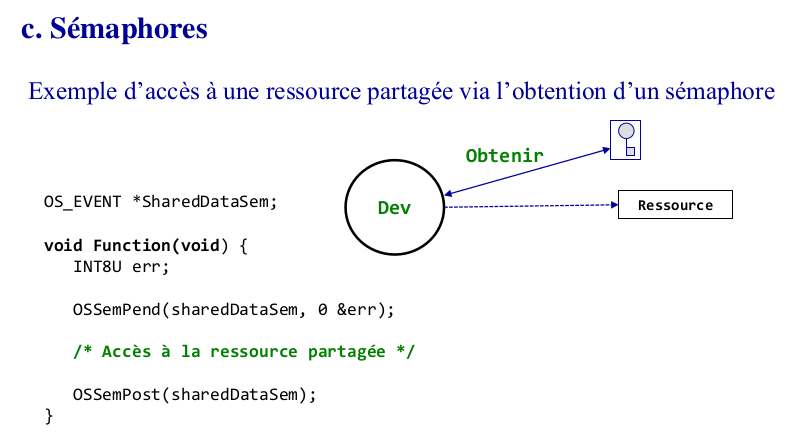
\includegraphics[width=8cm, height = 8cm, keepaspectratio]{Images/semaphore_ressource.png}
    	\caption{Exemple d'un utilisation de Sémaphore pour le partage d'un ressource sensible}
    	\label{fig:SemaphoreRessource}
    \end{figure}
    
    \paragraph{Deadlock} Il se peut que l'utilisation de sémaphore introduise des effets indésirabl.\\
    
    \begin{figure}[!ht]
    	\centering
    	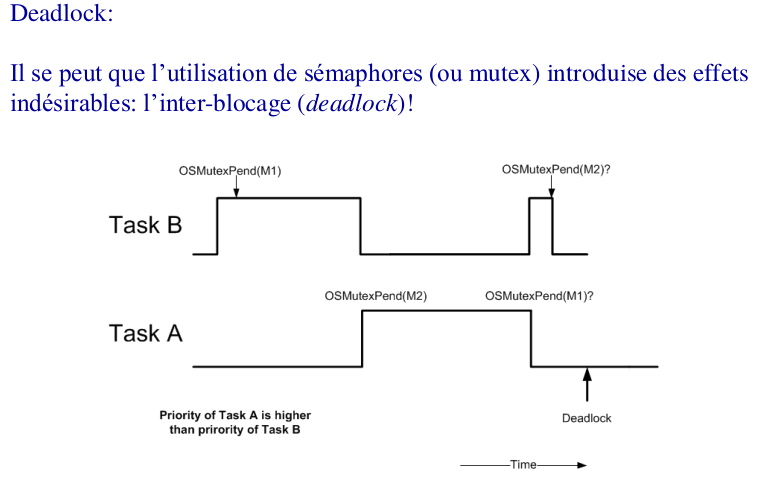
\includegraphics[width=8cm, height = 8cm, keepaspectratio]{Images/deadlock.png}
    	\caption{Exemple d'un deadlock}
    	\label{fig:Deadlock}
    \end{figure}
    
    Dans l'éventualité ou deux tâches veulent avoir un mutex détenus par une autre tâches, les deux tâches vont attendre éternellement. il convient alors aux tâches :
    
    \begin{itemize}
        \item Acquérire toutes les ressources avant de procédéer
        \item Acquérire les ressources dans le même ordre
        \item Relâcher les resource dans le même ordre
    \end{itemize}

    
    
    Les sémaphores peuvent aussi être utiliser our synchroniser des tâches. On appelle sa un rendez-vous unilatéral/bilatéral. uni/bi pour le nombre de tâches à synchroniser.\\
    
    \begin{figure}[!ht]
    	\centering
    	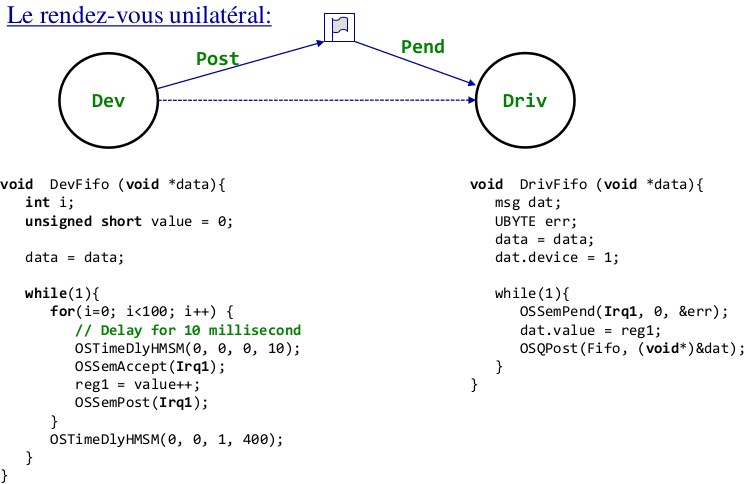
\includegraphics[width=8cm, height = 8cm, keepaspectratio]{Images/rdv_unilateral.png}
    	\caption{Exemple d'un rendez-vous unilateral}
    	\label{fig:Unilateral}
    \end{figure}
    
    \begin{figure}[!ht]
    	\centering
    	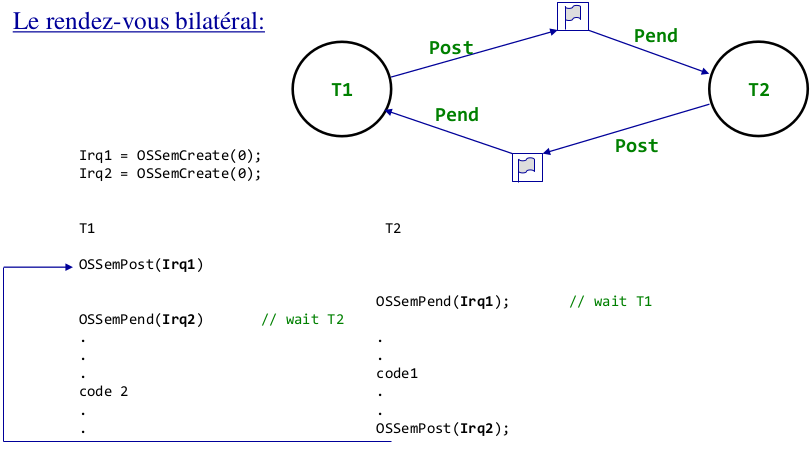
\includegraphics[width=8cm, height = 8cm, keepaspectratio]{Images/rdv_bilateral.png}
    	\caption{Exemple d'un rendez-vous bilateral}
    	\label{fig:Bilateral}
    \end{figure}
    
    On peut aussi utiliser les sémaphores à fin de synchroniser plusieurs tâches. Nous alons tous simplement avoir une registre qui contient plusieurs bit ou chaque bit représente l'état d'un sémaphore. On utilise un ou logique pour procéder. Dans ce cas, on peut même les appeller des flags.\\
    
    La communication entre plusieurs tâches se fait via des variables partagés. Les OS offre normalement des fonctionnalités de 'mailbox' ou de 'queues' INSÉRÉ SLIDE 68\\
    
    \subsubsection{Gestion des interruptions}
    l'interruption est un mécanisme matériel utilisé pour informer le processeur qu'un événement asynchrone à lieu.\\
    
    les interruptions peuvent être synchrone (logiciel) ou asynchrone (externes). Les interruptions peuvent être activer ou désactiver.\\
    
    Des interruptions externe permet à un processeur de traiter les événement lorsqu'ils surviennent plutôt que de poller continuellement sa venu (une boucle while)\\
    
    synchrone = de l'intérieur du processeur ; asynchrone = à l'extérieur du processur\\
    
    Évidemment, les interruptions peuvent être imbriqués\\
    
    Normalement nous allons avoir un compteur d'imbrications.\\
    
    En traitant un interruption, nous devons inévitablement changer de contexte. Pour faire cela, le processeur sauvegarde la valeur de toute les registres (stack) et retourne à cette états après avoir traite l'interruption.\\
    
    Le choix de la tâche à traiter dépend de la nature préemptive du noyau. Dans un système préemptif, sa fait en sorte qu'en sortant d'une interruption on n'est pas nécessairement obliger de retourner à la tâche qu'on exécutait avant de passer à l'ISR.\\
    
    \subsubsection{Problème d'inversion de priorité}
    Dans le cas ou la tâche moins prioritaire bloque la tâche prioritaire en raison du manque de resources/sémaphores, on inverse les priorités entre les tâches pour pouvoir libérer les resources.\\
    
    \begin{figure}[!ht]
    	\centering
    	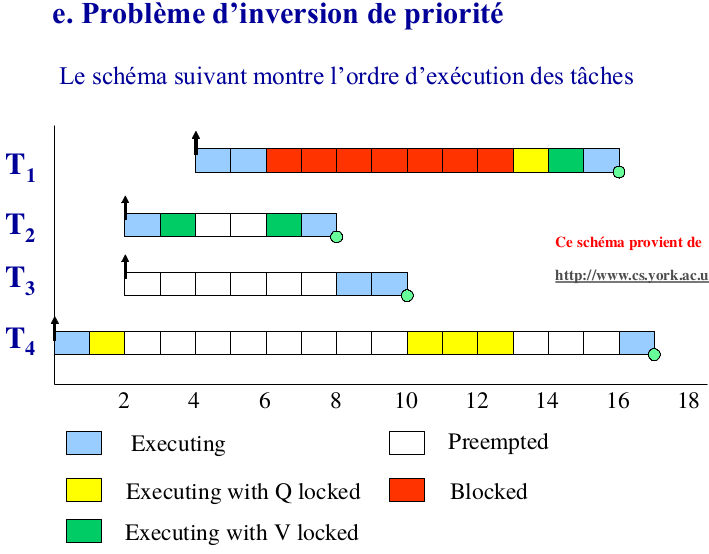
\includegraphics[width=8cm, height = 8cm, keepaspectratio]{Images/prob_scheduling.png}
    	\caption{Exemple du problème typique de scheduling}
    	\label{fig:Scheduling}
    \end{figure}
    
    Normalement, la tâche prioritaire aurait du s'exécuter en premier sauf que la tâche T4 avait un lock sur le mutex de la resource Q. Pour régler le problème, on utilise \textbf{héritage de priorité} pour pouvoir régler le problème. Pour faire cela, on change la priorité entre T1 et T4 temporairement pour que T4 relâche les ressources nécessaire pour ensuite rechanger les priorités\\
    
    \begin{figure}[!ht]
    	\centering
    	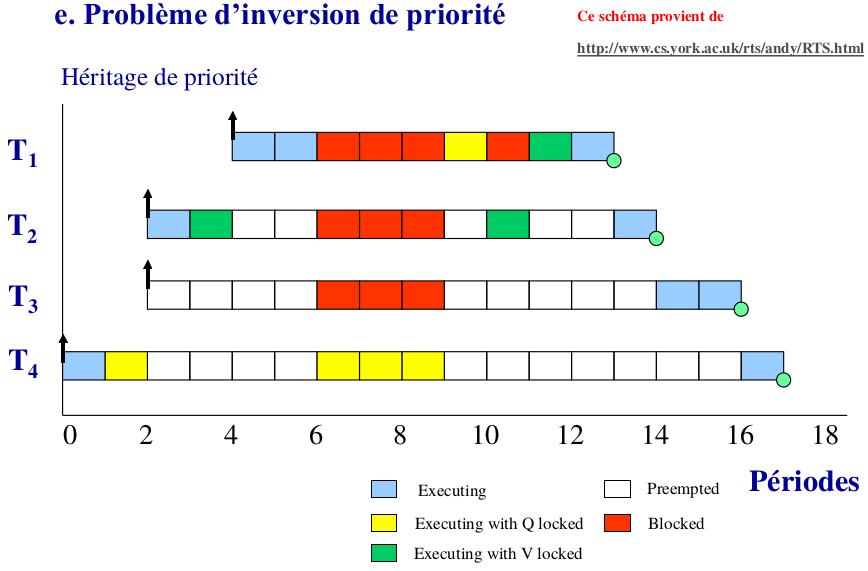
\includegraphics[width=8cm, height = 8cm, keepaspectratio]{Images/heritage_priorite.png}
    	\caption{Exemple de l'héritage des priorités}
    	\label{fig:HeritagePriorite}
    \end{figure}
    
    au final, après l'héritage de priorité, T1 s'est exécuter en 9 périodes vs 12.\\
    
    d'autre méthode peuvent aussi être utiliser. Comme par exemple l'ICPP:\\
    
    \begin{figure}[!ht]
    	\centering
    	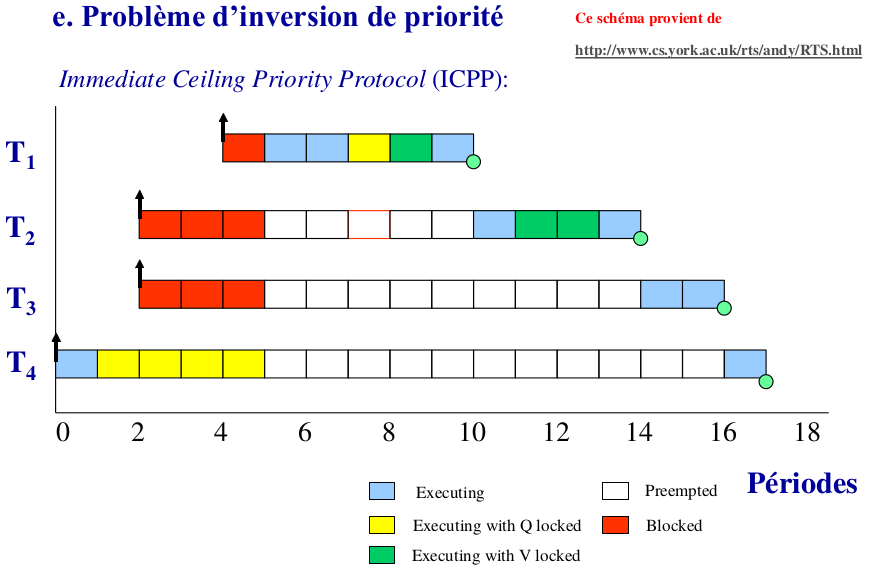
\includegraphics[width=8cm, height = 8cm, keepaspectratio]{Images/icpp.png}
    	\caption{Exemple de le l'ordonnancement fait par une heuristique d'ICPP}
    	\label{fig:ICPP}
    \end{figure}
    
    l'ICPP:\\
    \begin{itemize}
        \item minimise le temps de blocage
        \item demande peu de changements de contexte
        \item évite les problèmes d'inter-blocage (deadlock)
    \end{itemize}
    
    
    
    
\end{document}
